\documentclass[a4paper,11pt]{article}
\usepackage{graphicx}
\usepackage{enumerate}

\begin{document}

\begin{flushright}

\vspace{1.1cm}

{\bf\Huge Problem Set 5}

\rule{0.25\linewidth}{0.5pt}

\vspace{0.5cm}
%Put Authors
Justin Ely
\linebreak
\newline
%Put Author's affiliations
\footnotesize{605.411 Foundations of Computer Architecture \\}
\vspace{0.5cm}
% Date here below
04 October, 2016
\end{flushright}

\noindent\rule{\linewidth}{1.0pt}

%%%%%%%%%%%%%%%%%%%%%%%%%%%%%%%%%%%%%%%%%%%%%%%%%%%%%%%%%%

\section*{1)}
An r-type instruction goes through the states: 0, 1, 6, 7, before returning back to 0.  From the values given in the slides, 
the control values and next step codes in sequence are shown below. \\

\begin{tabular}{| c | c | c |}
  \hline	
       Step & Control & Next  \\  \hline
       0 & 1001010000001000 & 0001  \\  \hline
       1 & 0000000000011000 & 0110  \\  \hline
       6 & 0000000001000100 & 0111  \\  \hline
       7 & 0000000000000011 & 0000  \\  \hline
\end{tabular} \\

\noindent In hex, this sequence would be:  0x94081, 0x00186, 0x00447, 0x00030.


%%%%%%%%%%%%%%%%%%%%%%%%%%%%%%%%%%%%%%%%%%%%%%%%%%%%%%%%%%

\section*{2)} 
\begin{itemize}
 \item r-type
 \item load word
\end{itemize}

%%%%%%%%%%%%%%%%%%%%%%%%%%%%%%%%%%%%%%%%%%%%%%%%%%%%%%%%%%

\section*{3)}
\begin{tabular}{| c | c | c | c | c | }
  \hline	
       A & B & X  & Min-term & Max-term \\  \hline
       0 & 0 & 1 & A`B` & \\  \hline
       1 & 0 & 0 & & A` + B\\  \hline
       0 & 1 & 0 & & A + B`\\  \hline
       1 & 1 & 1 & AB & \\  \hline
\end{tabular} \\

\begin{figure}[h]
\caption{PLA for problem 3.}
\centering
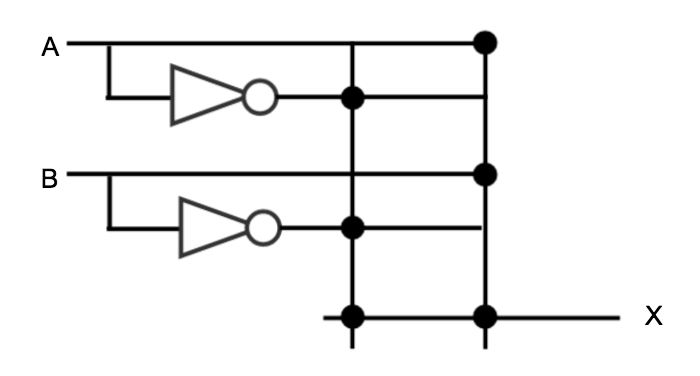
\includegraphics[width=.7\textwidth]{problem_3_pla.png}
\end{figure}


%%%%%%%%%%%%%%%%%%%%%%%%%%%%%%%%%%%%%%%%%%%%%%%%%%%%%%%%%%

\section*{4a)}
\begin{tabular}{| c | c | c | c |}
  \hline	
   000100 & 00000 & 00100 & 0000000000001010 \\  \hline
\end{tabular} \\

The op-code says this is a BEQ (I-type) instruction.  BEQ goes through states 0, 1, 8 on the state diagram.

\section*{4b)}
0, 1, 2, 6, 8

\section*{4c)}
\begin{itemize}
  \item Step 0: ALUSrcA = 0, ALUSrcB = 01, ALUOp = 00
  \item Step 1: ALUSrcA = 0, ALUSrcB = 11, ALUOp = 00
  \item Step 2: ALUSrcA = 1, ALUSrcB = 10, ALUOp = 00
  \item Step 6: ALUSrcA = 1, ALUSrcB = 00, ALUOp = 10
  \item Step 8: ALUSrcA = 1, ALUSrcB = 00, ALUOp = 01
\end{itemize}

\section*{4d)}
\begin{itemize}
  \item Step 0: ALU1 = PC, ALU2 = 4
  \item Step 1: ALU1 = PC, ALU2 = shift-by-two unit output
  \item Step 2: ALU1 = Register A, ALU2 = sign-extension unit output
  \item Step 6: ALU1 = Register A, ALU2 = Register B
  \item Step 8: ALU1 = Register A, ALU2 = Register B
\end{itemize}

\section*{4e)}
The branch is comparing register \$0 to register \$4.  Since \$0 = \$4 = 0, the branch is taken.  The new PC value will be
PC + 4 + (I-value $<$ $<$ 2) = 0000 0000 0100 0000 0000 0000 0010 1100.


%%%%%%%%%%%%%%%%%%%%%%%%%%%%%%%%%%%%%%%%%%%%%%%%%%%%%%%%%%

\section*{5)}
\begin{tabular}{| c | c | c | c | c | c | c | c | c | }
  \hline	
       X2 & X1 & X0  & a & b & c & d & minterm & maxterm \\  \hline
       0 & 0 & 0  &  &  & y &   & X2`X1`X0` & X2 + X1 + X0 \\  \hline
       1 & 0 & 0  &  & y &  & y & X2X1`X0` & X2` + X1 + X0  \\  \hline
       0 & 1 & 0  &  & y & y &   & X2`X1X0` & X2 + X1` + X0 \\  \hline
       1 & 1 & 0  & y &  &  &  y & X2X1X0` & X2` + X1` + X0 \\  \hline
       0 & 0 & 1  &  & y & y &   & X2`X1`X0 & X2 + X1 + X0` \\  \hline
       1 & 0 & 1  & y &  &  &  y & X2X1`X0 & X2` + X1 + X0` \\  \hline
       0 & 1 & 1  & y &  & y &   & X2`X1X0 & X2 + X1` + X0` \\  \hline
       1 & 1 & 1  &  &  &  &  y & X2X1X0 & X2` + X1` + X0` \\  \hline
\end{tabular} \\

\section*{5a)}
X = (X2X1X0') + (X2X1`X0) + (X2`X1X0)

\section*{5b)}
X = (X2X1`X0`) + (X2`X1X0`) + (X2`X1`X0)

\section*{5c)}
X = (X2`X1`X0`) + (X2`X1X0`) + (X2`X1`X0) + (X2`X1X0)

\section*{5d)}
X = (X2X1`X0`) + (X2X1X0`) + (X2X1`X0) + (X2X1X0)

%%%%%%%%%%%%%%%%%%%%%%%%%%%%%%%%%%%%%%%%%%%%%%%%%%%%%%%%%%

\section*{6)}
See figure below.

\begin{figure}[h!]
\caption{PLAs for problem 6.  Top to bottom: 5a, 5b, 5c, 5d}
\centering
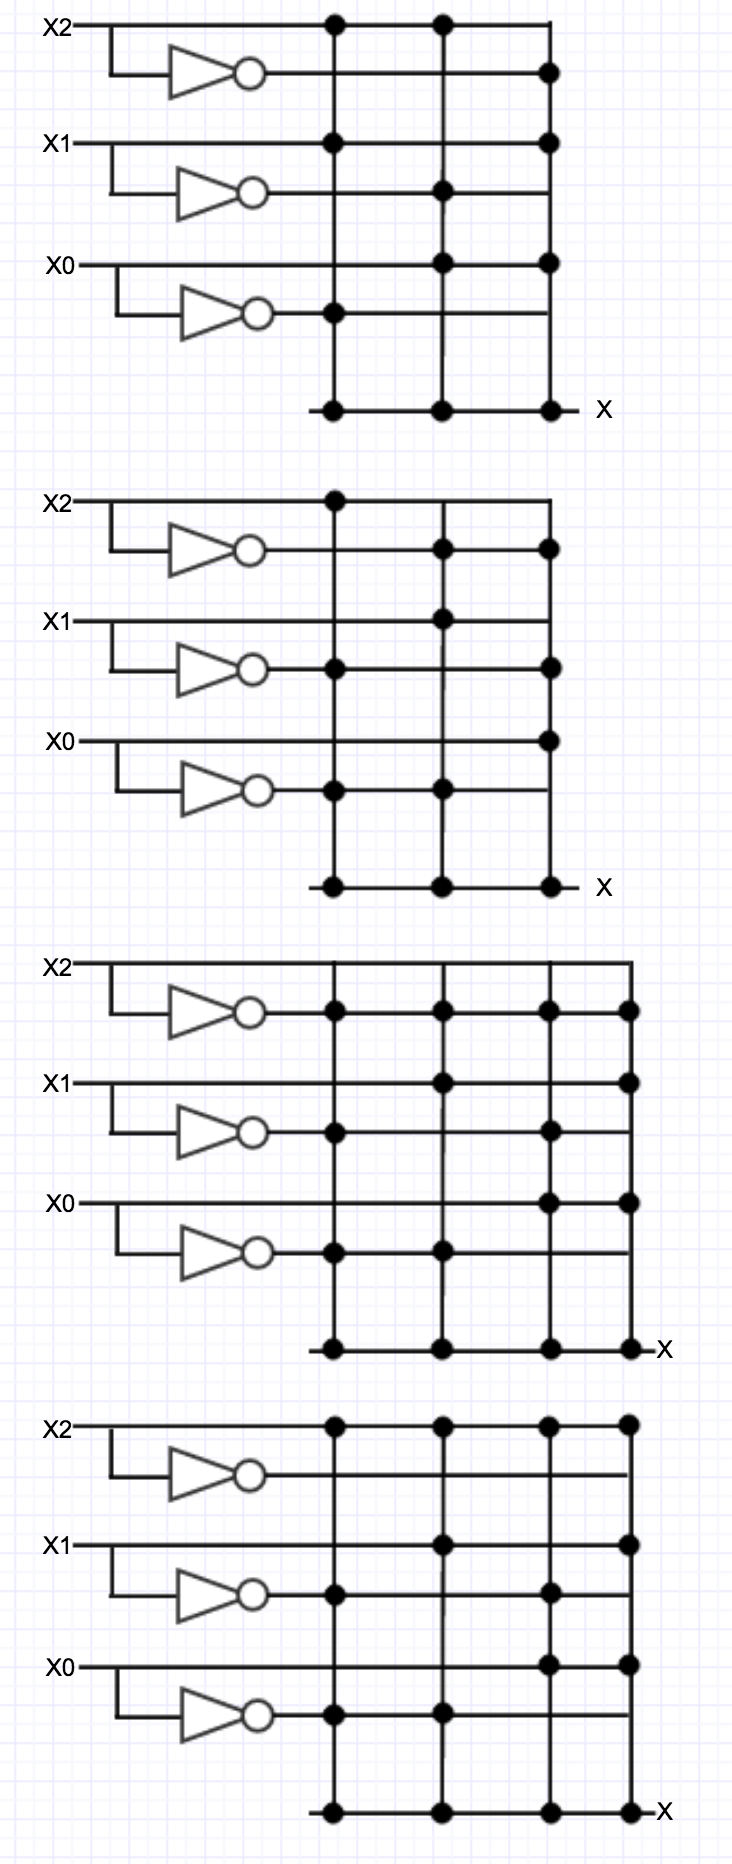
\includegraphics[width=.7\textwidth]{hw4_p6.png}
\end{figure}


%%%%%%%%%%%%%%%%%%%%%%%%%%%%%%%%%%%%%%%%%%%%%%%%%%%%%%%%%%

\section*{7)}
From the state diagram given in the lectures:\\

\begin{itemize}
  \item beq: 3
  \item j: 3
  \item or: 4
  \item add: 4 
  \item lw: 5
  \item sw: 4
  \item bne: 3
\end{itemize}


%%%%%%%%%%%%%%%%%%%%%%%%%%%%%%%%%%%%%%%%%%%%%%%%%%%%%%%%%%

\section*{8)}
\begin{itemize}
  \item lw \$2,40(\$4):  Uses the memory system when it is retrieving the specified word, the ALU to calculate the address, and the register file to see in which register to write the loaded word.
  \item add \$3,\$6,\$7: Uses the ALU do perform the arithmetic, and the register file to read operands and write result.
  \item slt \$5,\$6,\$7:  Uses the ALU to check if one register is less than another, and the register file to read operands and set the result.
  \item sw \$6,44(\$4):  Uses the register file and ALU to retrieve and calculate the address in memory to put the register value.
  \item and \$9,\$11,\$10:  Uses the ALU to perform the AND operation, and the register file to read operands and write result.
  \item or \$21,\$27,\$8: USes the ALU to perform the OR operation, and the register file to read operands and write result.
\end{itemize}

%%%%%%%%%%%%%%%%%%%%%%%%%%%%%%%%%%%%%%%%%%%%%%%%%%%%%%%%%%

\end{document}
